\documentclass[a4paper, 12pt]{article}
\usepackage{float}
\usepackage[T1]{fontenc}
\usepackage[utf8]{inputenc}
\usepackage[french]{babel} 
\usepackage[top=2.5cm, bottom=2.5cm, left=2.5cm, right=2.5cm]{geometry}
\usepackage{setspace}
\usepackage{graphicx}
\usepackage{hyperref}
\usepackage{longtable}


\begin{document}
    \begin{titlepage}
        \begin{center}
            \vspace*{1cm}

            
\includegraphics[scale=0.07]{../../exigences/png/logo-color.png}

            \vspace{0.8cm}
            \Huge
            \textbf{Heritage}

            \vspace{0.5cm}
            \LARGE
            Compte Rendu de Travail 1 \\
            05/05/2023

            \vspace{1.5cm}

            \textbf{Aloys LANA}

            \vfill
            \Large
            Travail d'Étude et de Recherche pour le Master 1 Informatique, parcours Données et Systèmes
            Connectés.\\

            \vspace{1cm}
            \large
            Université Jean Monnet, Saint Étienne, 2023
        \end{center}
    \end{titlepage}

    \tableofcontents

    \newpage
    \section{Résumé de la Semaine}
    Cette première semaine de travail a surtout consisté à la mise en place des bases du projet.
    J'ai donc mis en place la structure des documents et commencer la rédaction de ces derniers. 
    Voici donc un court résumé des tâches accomplies en sachant que cette semaine a été moins productive que ne le seront les prochaines puisque j'ai commencé mon travail estival et qu'il a fallut que je trouve mon rythme :
    \begin{itemize}
        \item Rédaction de l'Introduction et de la Description Générale du Document de Spécification des exigences.
        \item Planification du projet avec la réalisation d'un diagramme de Gantt.
        \item Création du Projet Angular et Experimentation autour du framework Angular et de son lien avec Spring Boot.
        \item Recherche concernant les API permettant de récupérer un livre en fonction de son ISBN, genre, auteur, etc...
    \end{itemize}

    \section{Planification du Projet}
    Durant ce projet je travaillerai en méthode agile avec des sprints de 3 semaines. L'objectif du premier sprint sera d'avoir un système de base (Base de Données, Authentification, Communication avec l'API) fonctionnel sur lequel on pourra s'appuyer ensuite pour ajouter les nouvelles fonctionnalités.
    \\
    Voici donc le Diagramme de Gantt prévisionnel de ce premier sprint :
    \\
    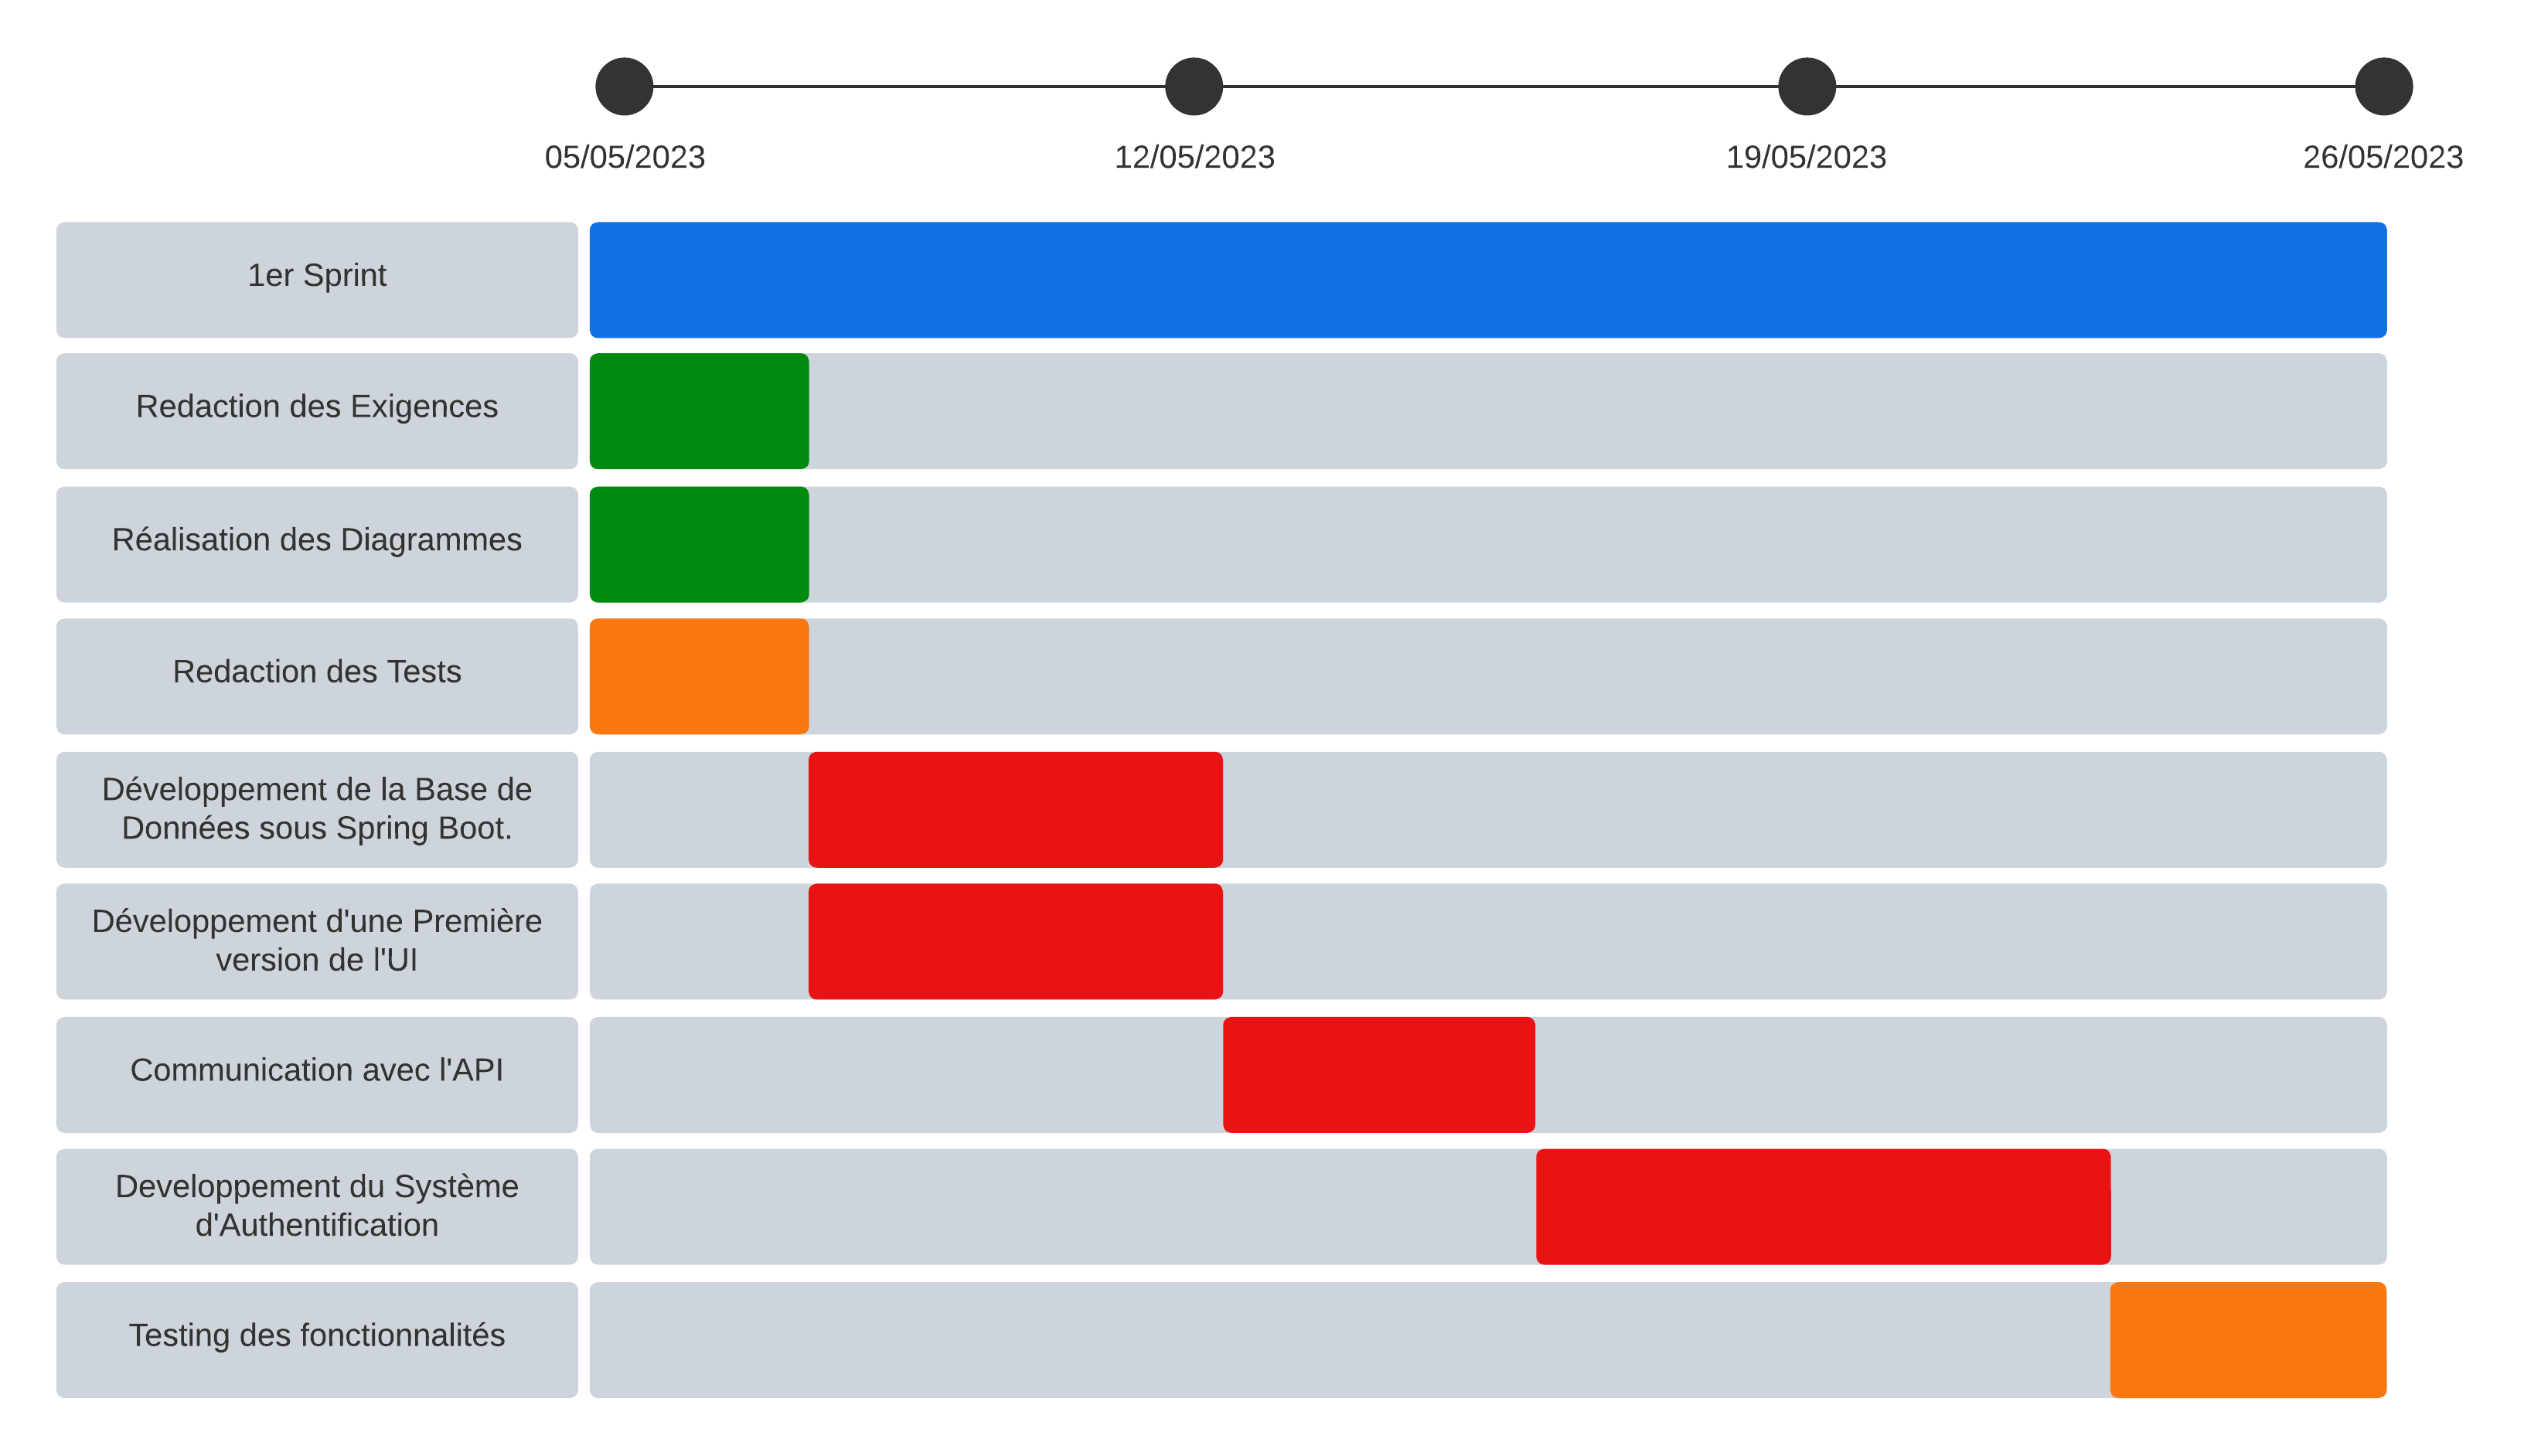
\includegraphics[scale=0.6]{Diagramme de Gantt Sprint 1.png}

    \section{Planification de la semaine a venir}
    Concernant la semaine de travail à venir je vais donc procédé à la rédaction des exigences liées au premier sprint, puis débuter le développement de la Base de Données sous Spring et d'une première interface utilisateur permettant de tester son fonctionnement.

\end{document}